\documentclass{mipt-thesis-bs}
\usepackage{mipt-thesis-biblatex}
\usepackage[justification=centering]{caption}
\usepackage{glossaries}
\usepackage{url}
\usepackage{pdfpages}
\usepackage{hyperref}
\usepackage[title]{appendix}
\usepackage{listings}
\addbibresource{ref.bib}


\begin{document}

\chapter{Адаптированный алгоритм Роббинса-Монро к задаче спуска к параметру бернуллевской величины, заданной логистической регрессией}


Ключевым результатом работы является предложение алгоритма обновления сложности $d$, обеспечивающего оптимальную сходимость вероятности решения задачи $s$ к методически рекомендованной $s^*$.

Приложение содержит: \begin{enumerate}
    \item краткое описание постановки и предметный обзор
    \item предложенный алгоритм, определяющий оптимальные параметры спуска  
    \item численный эксперимент, сравнивающий предложенный 
\end{enumerate} 

\section{Предметный обзор}

Постановка представляет тест как стохастический ряд вида $\{x\}_{t=0}$ каждый элемент, которого является случайной бернуллевской величиной с параметром $s$. 
Для ввода управляющей переменной задается сложность задачи $d$, параметризующий в совокупности с функцией отклика учащегося $f$, переменную $s_t = f(d)$.

 Таким образом, задача алгоритма предложить функцию $f(d_{t+1}^t,{x}_{i=0}^t)$, обеспечивающую оптимальную сходимость $\lim_{t \rightarrow \infty} \rho(s(d_t),s^*) =1$ согласно условиям:
 \begin{itemize}
    \item метрика $\rho(x,x') = (x-x')^2$ евклидова
    \item предполагается наличие банка $W$, возвращающего задачу произвольной сложности $d$
    \item функция отклика $f(d_t)$ ограничена числом $M$ и монотонно убывает
\end{itemize}

Алгоритм, отвечающий заданным требования  был предложен в работе \cite{yazidi2020balanced}. Авторы предложили правило обновления сложности:

\begin{equation}
    d_{t+1} = \Pi(d_t+\lambda (x(t) -s^*)),
    \label{yazidi}
\end{equation}
где функция $\Pi$ является ограничивающим оператором вида
\begin{equation}
    \Pi_H(d) = \left\{
        \begin{array}{ll}
            d,\ \text{прт}\ 1<d<0 \\
            1,\ d\ge 1\\
            0, \text{при} \ d \le 0\\
        \end{array}
    \right.
\end{equation}

Алгоритм по форме соответствует алгоритму Роббинса-Монро\cite{robbins1951stochastic}, известному в теории стохастической аппроксимации. 
Отметим, что поскольку коэффициент $\lambda$ является постоянной, то сходимость по алгоритму Роббинса-Монро не гарантируется.

\textit{\textbf{Теорема.} Алгоритм Роббинса-Монро}. Алгоритм, выполняющий пересчет по правилу $d_{n+1} =d _n + a_d(s^*-s)$ сходится в $L^2$ норме при выполнении \begin{enumerate}
    \item значения функции отклика монотонны и $s$ ограничены: $\exists N\ \forall x : | s(x) | \le N$
    \item $\sum_{t=0}^\infty a_t = \infty$
    \item $\exists M : |\sum_{t=0}^\infty a_t^2 |< M$.
\end{enumerate}

Доказательство теоремы приведено в аппендиксе работы \ref{monro}.

Если функция отклика $s$ строго выпукла и дважды дифференцируема,
то асимптотическая скорость сходимости равна $\mathcal{O}(\frac{1}{n})$ \cite{sacks1958asymptotic}.

Выбор коэффициент $a_n$ существенно образом влияет на число шагом сходимости последовательности.
Авторы оригинального алгоритма предлагают $a_n = \frac{\lambda}{n}$. В работах \cite{lai1979adaptive}
используется альтернативный подход, исходящий из \begin{enumerate}
    \item несмещенности оценки $\mathrm{E}d_n=d$.
    \item минимизации дисперсии $\mathbf{D} d_n=0$.
\end{enumerate}
Современный подход направлен на учетом априорного представления в виде нормального распределения \begin{enumerate}
    \item нормальным распределением \cite{joseph2004efficient}
    \item многомерных биноминальных распределений \cite{xiong2018efficient}
    \item цепи гауссовых распределений \cite{liu2024robbins}.
\end{enumerate}
Подвергается изменениям и сама схема доказательства как в работе \cite{joseph2004efficient}.
Автор предлагает заменить оптимизируемый коэффициент $s^*$ на параметр $b_n$:
$$
    x_{n+1} = x_{n} - a_n(x -b_n).
$$
Существенный вклад в развитие методов стохастической аппроксимации внёс Борис Теодорович Поляк \cite{polyak1990new},
предложивший метод усреднения управляющего параметра $s$:
\begin{equation}
    \hat{s}_{n+1} = \sum_{i=0}^n s_i.
    \label{polyak}
\end{equation}
    Такой подход позволяет подавлять
высокочастотные шумовые компоненты при аппроксимации ряда,
что позволяет использовать методы с большим шагом спуска.
Условия эффективной применимости состоят в малом изменении коэффициентов $a_n$:
\begin{equation}
   \frac{a_{n}-a_{n+1}}{a_{n}}=\mathit{o}(a_{n}).
   \label{polyak_assumptions}
\end{equation}

\section{Вклад}

Схема доказательства \begin{enumerate}
    \item используем модифицированный алгоритм Роббинса-Монро, используя 
    \item зададим связь между функцией отклика $s(d)$ и параметрами $a_n$ и $b_N$ через условия несмещенности оценки $E(x_n)$ и
минимизации дисперсии $\mathbf{D}(x_n) \rightarrow min$  \cite{hu1997strong} \cite{hu1998sequential}
    \item определим явное выражение $a_n$ и $b_n$ для априорного представления о функции отклика в виде параметрической модели Эло $s(d,\alpha,\beta) = 1 - \frac{1}{1+\exp\left(-\beta \cdot(\mathbf{d} -\alpha)\right)}$
\end{enumerate}

\begin{figure}[h!]
    \centering
    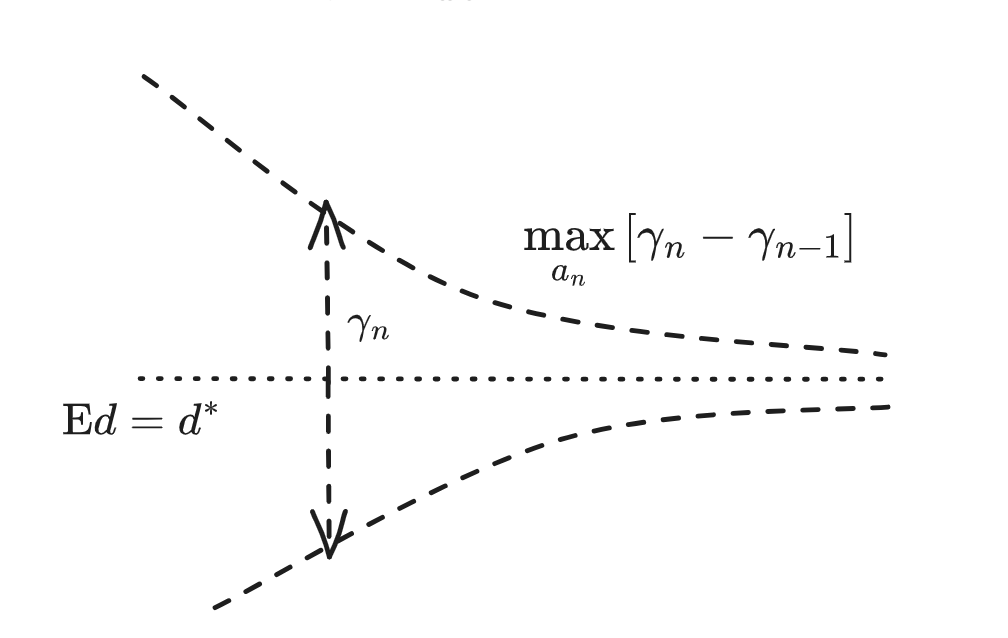
\includegraphics[width=0.5\textwidth]{assets/dispersion_reduction.png}
    \caption{Использование несмещенной оценки с постепенной редукцией дисперсии}
    \label{principal_scheme}
\end{figure}

\textit{\textbf{Теорема.}Адаптированный алгоритм Роббинса-Монро для случая наблюдений, имеющих бернуллевское распределение.} \label{algo} 
При условии $\forall n \hookrightarrow x_n \sim \text{Bern}(s(d_n))$ выполняются следующие утверждения. \begin{enumerate}
    \item Оптимальная сходимость достигается при $a_n = \frac{\mathbb{E}[d_n s(d_n)]}{\mathbb{E}s(d_n)(1 - \mathbb{E}s(d_n))}$ , $b_n =\mathbb{E} s(d_n)$
    \item Для функции отклика, представленной параметрической моделью Эло $s(d,\alpha,\beta) = 1 - \frac{1}{1+\exp\left(-\beta \cdot(d -\alpha)\right)}$
     и в предположении нормальности распределения $d \sim \mathcal{N}(\alpha,\sigma^2)$ получим аппроксимацию рядов $a_n$ и $b_n$, обеспечивающих оптимальную сходимость как\begin{itemize}
        \item $a_n = \frac{1}{b_n(1-b_n)} \frac{1}{4  \beta \sqrt{1+\frac{\pi\gamma_n^2}{8}}} \exp\left( \frac{- \pi (\alpha-d^*)^2}{16  \beta^2 ( 1+\frac{\pi\gamma_n^2}{8})}\right)$
        \item $b_n = \frac{1}{2} + \frac{1}{2} \text{erf}\left(\frac{\sqrt{\pi} (\alpha-d^*)}{4 \sqrt{1+\frac{\pi\gamma_n^2}{8}}} \right)$.
    \end{itemize} 
\end{enumerate}
\textit{Доказательство}
Сходимость метода приведена в аппендиксе работы \ref{ino}.
1) Используем рекуррентное представление для поиска оптимальных параметров $a_n,b_n$
\begin{equation}
    d_{n+1} = d_n -  a_n(x_n-b_n).
    \label{mod_scheme}
\end{equation}
Рассчитаем матожидание $\mathrm{E}_{d_n ~ p(d_n)}$ как:
\begin{equation}
    \mathrm{E} d_{n+1} = \mathrm{E} d_n -  a_n(\mathrm{E}x_n-b_n).
\end{equation}
Запишем условия $\mathrm{E} d_{n+1} = d^*$ c учетом $\mathrm{E} d_{n} = \dots \mathrm{E} d_{1}= d^*$:
\begin{equation}
    a_n (\mathrm{E} s(d_n) - b_n)  =0.
\end{equation}
Следовательно,
\begin{equation}
    \label{b_n}
    b_n = \mathrm{E} s(d_n).
\end{equation}
Коэффициент $a_n$ найдем из минимизации дисперсии $\mathbf{D} d_{n+1}$. Запишем $\mathbf{D}_{x_n \sim Bern(x | s(d_n))}$ для выражения \ref{mod_scheme}:
\begin{equation}
    \label{disp}
    \mathbf{D} d_{n+1} = \mathbf{D} d_n + a_n^2 \mathbf{D} (x_n-b_n)  - 2 a_n \mathrm{E}\left[(x_n-b_n)d_n\right].
\end{equation}
Поскольку $x_n \sim \text{Bern}(s(d_n))$,то
\begin{equation}
    \mathbf{D}(x_n-b_n) = \mathrm{E} s(d_n) \mathrm{E} (1-s(d_n))=  \mathrm{E} s(d_n)  (1-\mathrm{E}s(d_n)).
\end{equation}
С учетом $b_n = \mathrm{E} s_d$ и $\mathrm{E} d_n =d^*$:
\begin{equation}
    \mathrm{E}\left[(x_n-b_n)d_n\right] = \mathrm{E}\left[x_n d_n \right] - b_n  \mathrm{E} d_n = \mathrm{E} \left[s(d_n) d_n\right] - \mathrm{E} s(d) d^*.
\end{equation}
Тогда:
\begin{equation}
    \mathbf{D} d_{n+1} = \mathbf{D} d_n + a_n^2 \mathrm{E}s(d_n)\mathrm{E}(1-s(d_n)) - 2 a_n \mathrm{E}\left[ s(d_n) (d_n-d^*)\right].
\end{equation}
Из условия $\frac{\partial \mathbf{D}{d_{n+1}}}{\partial a_n} =0 $ получаем:
\begin{equation}
    \label{diff}
    a_n = \frac{\mathrm{E} \left[ (d_n-d^*) s(d_n)\right]}{\mathrm{E}s(d_n)(1 - \mathrm{E}s(d_n))}.
\end{equation}
Тогда связь между дисперсиями на каждом шаге запишется как:
\begin{equation}
    \mathbf{D} d_{n+1} = \mathbf{D} d_n - \frac{\left(\mathrm{E} \left[ (d_n-d^*) s(d_n)\right] \right)^2}{\mathrm{E}s(d_n)(1 - \mathrm{E}s(d_n))} 
\end{equation}
2) Определим оптимальные коэффициенты $a_n$ и $b_n$ для случая отклика согласно модели Эло: $s(d_n) = \sigma(d,\alpha,\beta) = 1 - \frac{1}{1+\exp(-\frac{(d_n-\alpha)}{\beta})}$. Исходя из предположения $d^*$:
\begin{equation}
    d^* = \alpha  - \beta \log\left(\frac{s^*}{1-s^*}\right).
\end{equation}
Согласно условию $d$ распределен нормально $\sim \mathcal{N}(\alpha_n,\gamma_n)$. $\alpha_n = d^*$, исходя из несмещенности оценки $d_n$. $\gamma_n$ рекуррентно связан с значениям предыдущих операций согласно \ref{diff}:
\begin{equation}
    \label{gamma_connection}
    \gamma_n = \gamma_{n-1} - \frac{\left(\mathrm{E} \left[ (d_n-d^*) s(d_n)\right] \right)^2}{\mathrm{E}s(d_n)(1 - \mathrm{E}s(d_n))}.
\end{equation}
Найдем $b_n$ из \ref{b_n}:
\begin{equation}
    b_n = \int_{-\infty}^{\infty} s(x) \mathcal{N}_{d^*,\gamma_n}(x) d x = \int_{-\infty}^{\infty} \sigma(x,\alpha,\beta) \mathcal{N}_{d^*,\gamma_n} d x.
\end{equation}
Для этого используем аппроксимацию логнормальныого интеграла через функцию ошибки $\text{erf}(x) = \int_{-\infty}^x \exp(-t^2)$:
\begin{equation}
     \sigma(x, \alpha, \beta) \approx \frac{1}{2} + \frac{1}{2} \text{erf}\left(\frac{(x-\alpha)\sqrt{\pi}}{4 \beta}\right).   
\end{equation}
Свертка  $\text{erf}(x)$ c плотностью вероятности гауссового распределения $\mathcal{N}(d^*,\gamma_n)$ является табличным интегралом \cite{ng1969table}:
\begin{equation}
    b_n \approx \int_{-\infty}^{\infty} \left[\frac{1}{2} + \frac{1}{2} \text{erf}\left(\frac{\sqrt{\pi}}{4\beta} (x-\alpha) \right) \right] \mathcal{N}_{d^*,\gamma_n}(x) dx = 
    \frac{1}{2} + \frac{1}{2} \text{erf}\left(\frac{\sqrt{\pi} (\alpha-d^*)}{4 \beta \sqrt{1+\frac{\pi\gamma_n^2}{8}}} \right).
\end{equation}
Найдем $a_n$ из \ref{diff}:
\begin{equation}
    \label{a_n}
    \begin{aligned}
          a_n &= \frac{1}{b_n(1-b_n)} \int_{-\infty}^{\infty} d (\sigma(x\alpha,\beta) -d^*) \mathcal{N}_{d^*,\tau}(x)  dx \\  
          &\approx  \int_{-\infty}^{\infty} x \left[\frac{1}{2} - d^* + \frac{1}{2} \text{erf}\left(\frac{(x-\alpha)\sqrt{\pi}}{4 \beta}\right)\right] \mathcal{N}_{d^*,\gamma_n}(x) dx \\
          &= \frac{d*}{2 \gamma_n^2} \text{erf}\left(\frac{\sqrt{\pi} (\alpha-d^*)}{4 \sqrt{1+\frac{\pi\gamma_n^2}{8}}} \right)  + \frac{1}{4 \gamma_n^2} \frac{1}{b_n(1-b_n)} \int_{-\infty}^{\infty} x \text{erf}\left(\frac{(x-\alpha)\sqrt{\pi}}{4 \beta}\right) \exp\left(\frac{(x-d^*)^2}{2 \gamma_\frac{1}{b_n(1-b_n)}n^2}\right) dx \\
          & = \frac{d*}{2 \gamma_n^2} \text{erf}\left(\frac{\sqrt{\pi} (\alpha-d^*)}{4 \sqrt{1+\frac{\pi\gamma_n^2}{8}}} \right) + \frac{1}{4 \gamma_n^2} \frac{1}{b_n(1-b_n)} I(\alpha,\beta,d^*,\gamma_n).
    \end{aligned}
\end{equation}
Заметим, что полученный интеграл $I(\alpha,\beta,d^*,\gamma_n)$ можно связать с табличным  
$T(\alpha,\beta,d^*,\gamma_n) = \int\text{erf}\left(\frac{\sqrt{\pi}}{4\beta} (x-\alpha) \right) \exp\left(\frac{(x-d^*)^2}{2 \gamma_n^2}\right) dx$ через дифференцирование по параметру $d^*$: 
\begin{equation}
    \label{left}
    T'_{d^*} = - \frac{1}{2\gamma_n^2}I(\alpha,\beta,d^*,\gamma_n) + \frac{d*}{2 \gamma_n^2} \text{erf}\left(\frac{\sqrt{\pi} (\alpha-d^* \beta )}{4 \beta \sqrt{1+\frac{\pi\gamma_n^2}{8}}} \right) .
\end{equation}
C другой стороны:
\begin{multline}
    \label{right}
    \begin{aligned}
        T'_{d^*} &= \frac{1}{2} \text{erf}\left(\frac{\sqrt{\pi} (\alpha-d^*)}{4  \beta \sqrt{1+\frac{\pi\gamma_n^2}{8}}} \right)'_{d^*} = - \frac{2}{\sqrt{\pi} \beta} \frac{\sqrt{\pi}}{4 \sqrt{1+\frac{\pi\gamma_n^2}{8}}}
        \frac{1}{2} \exp\left( \frac{- \pi (\alpha-d^*)^2}{16  \beta^2 ( 1+\frac{\pi\gamma_n^2}{8})}\right) =\\
        &= - \frac{1}{4  \beta \sqrt{1+\frac{\pi\gamma_n^2}{8}}}
        \exp\left( \frac{- \pi (\alpha-d^*)^2}{16  \beta^2( 1+\frac{\pi\gamma_n^2}{8})}\right).
    \end{aligned}
\end{multline}
Приравнивая \ref{left} и \ref{right} получаем:
\begin{equation}
    \label{main_integral_solution}
    I= \frac{1}{4 \sqrt{1+\frac{\pi\gamma_n^2}{8}}} \exp\left( \frac{- \pi (\alpha-d^*)^2}{16 \beta^2 ( 1+\frac{\pi\gamma_n^2}{8})}\right) - \frac{d*}{2 \gamma_n^2} \text{erf}\left(\frac{\sqrt{\pi} (\alpha-d^*)}{4 \beta\sqrt{1+\frac{\pi\gamma_n^2}{8}}} \right).   
\end{equation}
Подставляем $I$ в \ref{a_n} получаем аппроксимацию ${a_n}$:
\begin{equation}
     a_n \approx \frac{1}{b_n(1-b_n)} \frac{1}{4  \beta \sqrt{1+\frac{\pi\gamma_n^2}{8}}} \exp\left( \frac{- \pi (\alpha-d^*)^2}{16  \beta^2 ( 1+\frac{\pi\gamma_n^2}{8})}\right).
\end{equation}
Также получим $\gamma_n$ из \ref{main_integral_solution} и \ref{gamma_connection}: 
\begin{equation}
    \gamma_n = \gamma_{n-1} - \frac{\gamma_{n-1}^2}{1+\gamma_{n-1}} \frac{1}{b_n(1-b_n)}
    \exp\left(\frac{- \pi (\alpha-d^*)^2}{16  \beta^2 ( 1+\frac{\pi\gamma_n^2}{8})})^2\right)^2.
\end{equation}
$\blacksquare$
\subsection{Адаптация к численному расчету}
Явно приведем ключевые выражения для численного выражения:
1) Приближение оптимального корня:
\begin{equation}
    d^* = \alpha  - \beta \log\left(\frac{s^*}{1-s^*}\right).
\end{equation}
2) Коэффициенты $a_n$, $b_n$, $\gamma_n$ рассчитываются рекурсивно
\begin{equation}
    \begin{aligned}
        &\gamma_n = \gamma_{n-1} - \frac{\gamma_{n-1}^2}{1+\gamma_{n-1}} \frac{1}{b_n(1-b_n)}
    \exp\left(\frac{- \pi (\alpha-d^*)^2}{16  \beta^2 ( 1+\frac{\pi\gamma_n^2}{8})})^2\right)^2 \\
        &a_n = \frac{1}{b_n(1-b_n)} \frac{1}{4  \beta \sqrt{1+\frac{\pi\gamma_n^2}{8}}} \exp\left( \frac{- \pi (\alpha-d^*)^2}{16  \beta^2 ( 1+\frac{\pi\gamma_n^2}{8})}\right)  \\
        &b_n = \frac{1}{2} + \frac{1}{2} \text{erf}\left(\frac{\sqrt{\pi} (\alpha-d^*)}{4 \beta \sqrt{1+\frac{\pi\gamma_n^2}{8}}} \right).\\  
    \end{aligned}
\end{equation}
Процедуру пересчета коэффициента можно выполнить до проведения испытания, тем самым ускорив исполнение программы.

\section{Описание численных экспериментов}
Численное моделирование исследует поведение предложенного алгоритма для функции логистической регрессии в сравнение с классическими подходам.
Исходный код на языке Python доступен в открытом репозитории диссертации
\footnote{\url{https://github.com/NMashalov/EducationGenerativeModelApplication}}.

Ключевым параметром для анализа является соотношение изменения параметра сложности задачи $\Delta d$ к параметру роста ${\beta}$.
\begin{figure}[h]
    \centering
    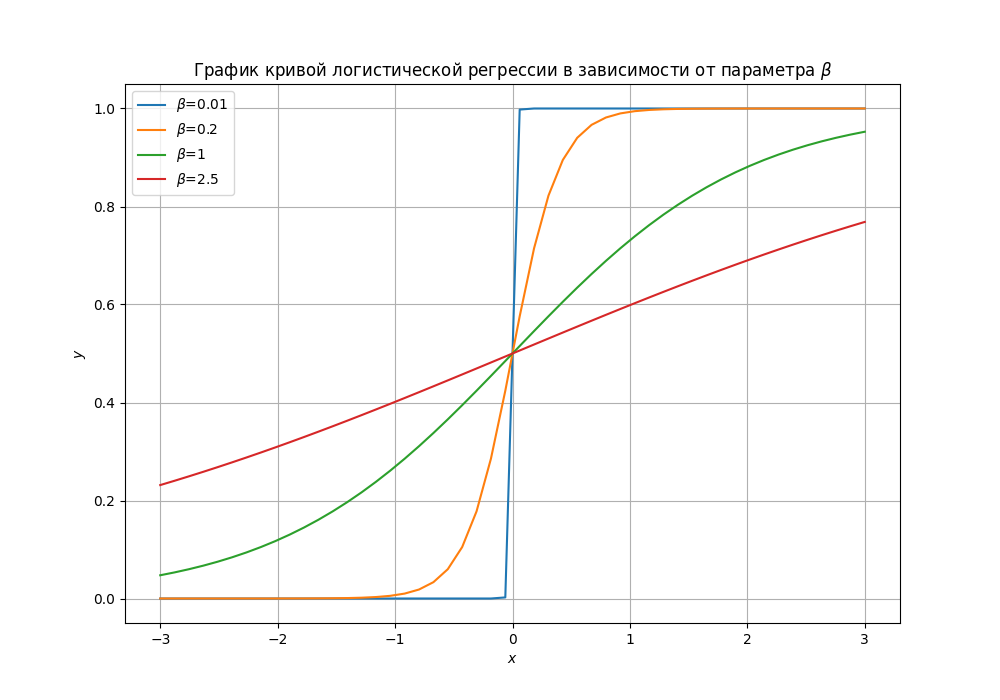
\includegraphics[width=0.8\textwidth]{assets/logistic.png}
    \caption{Демонстрация изменения графика логистической регрессии от параметр роста}
    \label{logistic_figure}
\end{figure}
Таким образом, были исследованы две ключевые краевые постановки: \begin{enumerate}
    \item малые изменения  $\Delta d / \beta \approx 0$ 
    \item значительные изменения $\Delta d / \beta \approx 1$ 
\end{enumerate}
В каждом эксперименте сравнивалась эффективность метода с классическим алгоритмом Роббинса-Монро и его аналогом с фиксированным коэффициент $\lambda$ как в работе \cite{yazidi2020balanced}. Дополнительно изучено влияние модификации по методу Поляка скользящим средним. 

Гладкие графики траекторий получается путем визуализации среднего и перцентилей распределения. Для их численного расчета используется метод бутстрэп.
Эксперимент проводится $B >> 1$ раз, после чего статистики считаются путем расчета распределения.   

В разделе приведены ключевые графики, полный набор доступен в приложении статьи. Отметим, что при анализе сходимости число шагов $N$ определяется аналогично правилу предела.
$N$ считается шагом достижения сходимости,
если все последующие точки не выходят за границу $\epsilon$.  $\epsilon$ выбирается индивидуально из соображений статистической значимости результата. 

\subsection{Случай $\Delta d / \beta \approx 1$ }
Эксперимент проводился для $s(d) = \frac{1}{1+\exp(-5(d-0.6))}$ c начальной сложность $d_0 =0.2$ и целевым параметром $s^* =0.4$
\footnote{Для наглядности в таблице классический алгоритм Роббинса-Монро сокращается до сокращения "Р.-М." с указанием параметра шага.}
\begin{figure}[h]
    \centering
    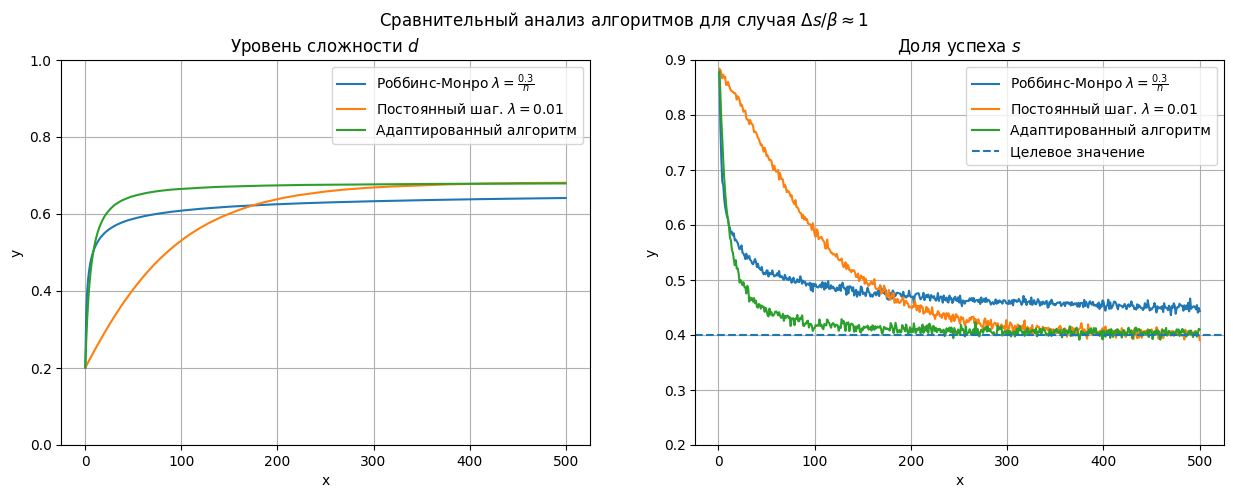
\includegraphics[width=1.0\textwidth]{assets/1/result.png}
    \caption{Предложенный алгоритм}
    \label{exp1:algo}
\end{figure}
Отметим также чувствительность алгоритм Роббинса-Монро к параметру шага. \ref{exp1:classic}
\begin{figure}[h]
    \centering
    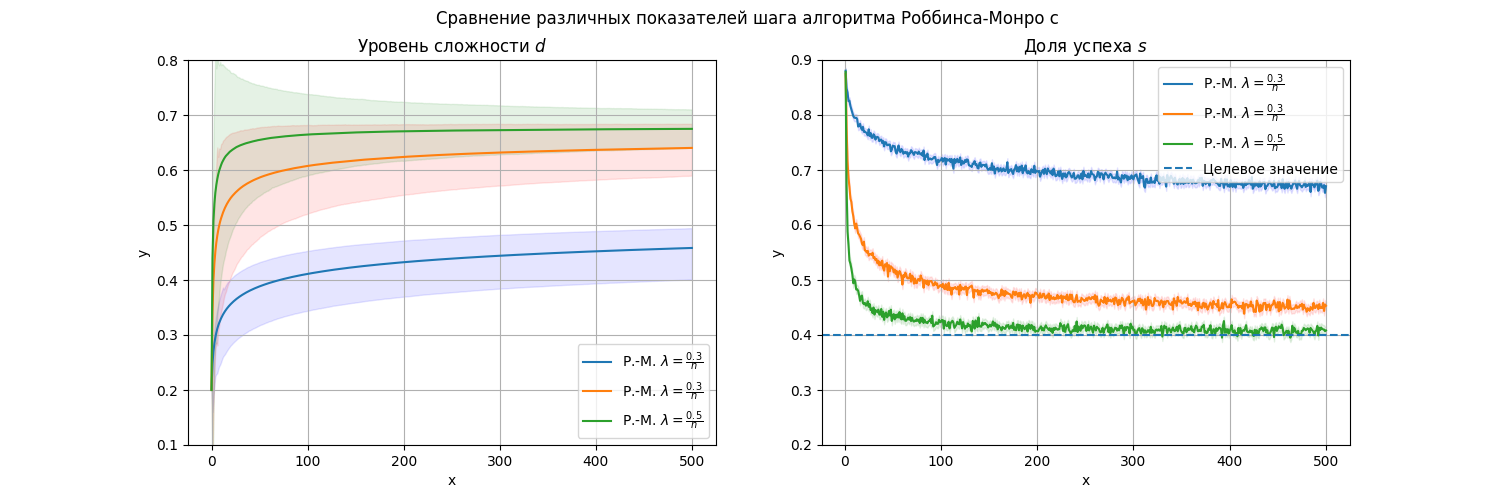
\includegraphics[width=1.0\textwidth]{assets/1/sensitivity.png}
    \caption{Классический алгоритм Роббинса-Монро чувствителен к параметру $\lambda$}
    \label{exp1:classic}
\end{figure}
\begin{table}
    \centering
    \begin{tabular}{ ||c | c|| }
        \hline 
          \text{Название алгоритма} &  \text{Число шагов}\\
        \hline 
         \text{Постоянный} $\lambda_n = 0.01$ & $400  \pm 20$ \\  
         \text{Алгоритм Р.-М.} $\lambda_n = 0.1$ & \text{Не сошелся} \\
         \text{Алгоритм Р.-М.} $\lambda_n = 0.5$ & $250 \pm 30$ \\
         \text{Адаптированный алгоритм Р.-М.} & $200 \pm 35 $   \\
         \hline
    \end{tabular}        
    \caption{Сравнение числа шагов сходимости в постановке $\Delta d / \beta \approx 1$}
    \label{exp1:table}
\end{table}
\subsection{Случай $\Delta d / \beta \approx 0$ }
Эксперимент проводился для $s(d) = \frac{1}{4(d-0.6)}$ c начальной сложность $d_0 =0.2$ и целевым параметром $s=0.8$. Число раундов было выбрано минимальным для

\footnote{Для наглядности в таблице классический алгоритм Роббинса-Монро сокращается до сокращения "Р-М" с указанием параметра шага.}

\begin{figure}[h]
    \centering
    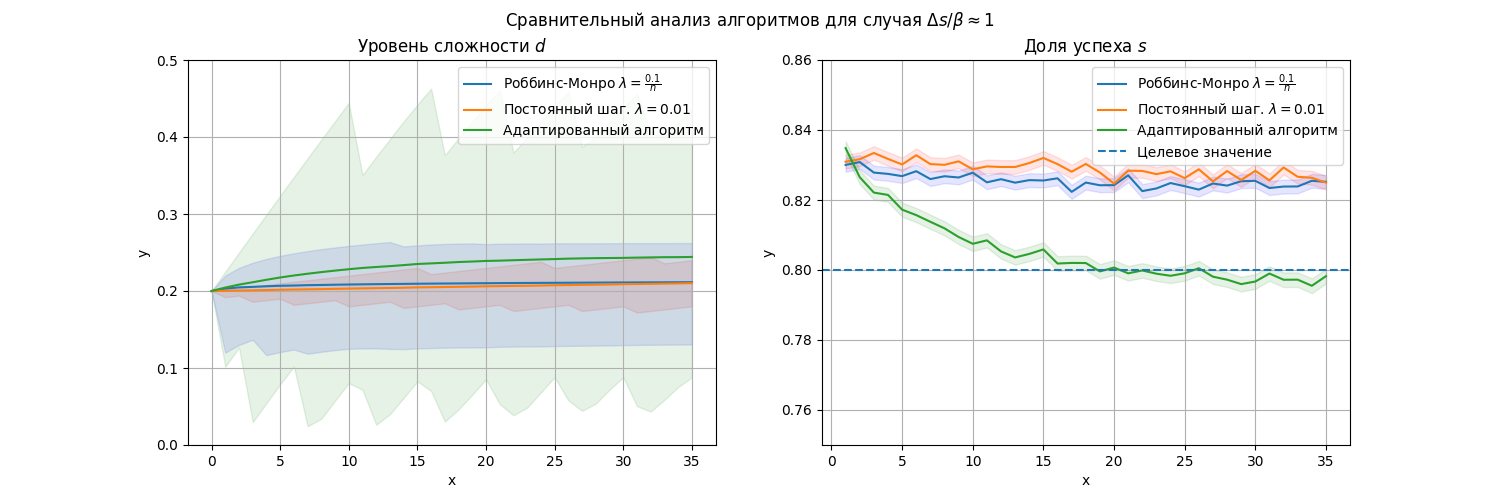
\includegraphics[width=1.0\textwidth]{assets/2/comparison_analysis.png}
    \caption{Предложенный алгоритм имеет высокую скорость реакции $d$}
    \label{exp2:сomparison}
\end{figure}

\begin{table}
    \centering
    \begin{tabular}{ ||c | c|| }
        \hline 
        \text{Название алгоритма} &  \text{Число шагов}\\
        \hline 
        \text{Постоянный} $\lambda_n = 0.01$ & $400  \pm 20$ \\  
        \text{Алгоритм Р.-М.} $\lambda_n = 0.1$ & \text{Не сошелся} \\
        \text{Алгоритм Р.-М.} $\lambda_n = 0.5$ & $250 \pm 30$ \\
        \text{Адаптированный алгоритм  Р.-М.} & $200 \pm 35 $   \\
        \hline
    \end{tabular}
    \caption{Сравнение числа шагов сходимости в постановке $\Delta d / \beta \approx 0$}
    \label{exp2:table}
\end{table}

\subsection{Случай значительного отличия априорных представлений о наклоне кривой от действительного}
Рассмотрен случай, в котором $\beta$ априорная значительно отличается $\beta^*$ действительного.
\begin{figure}[h]
    \centering
    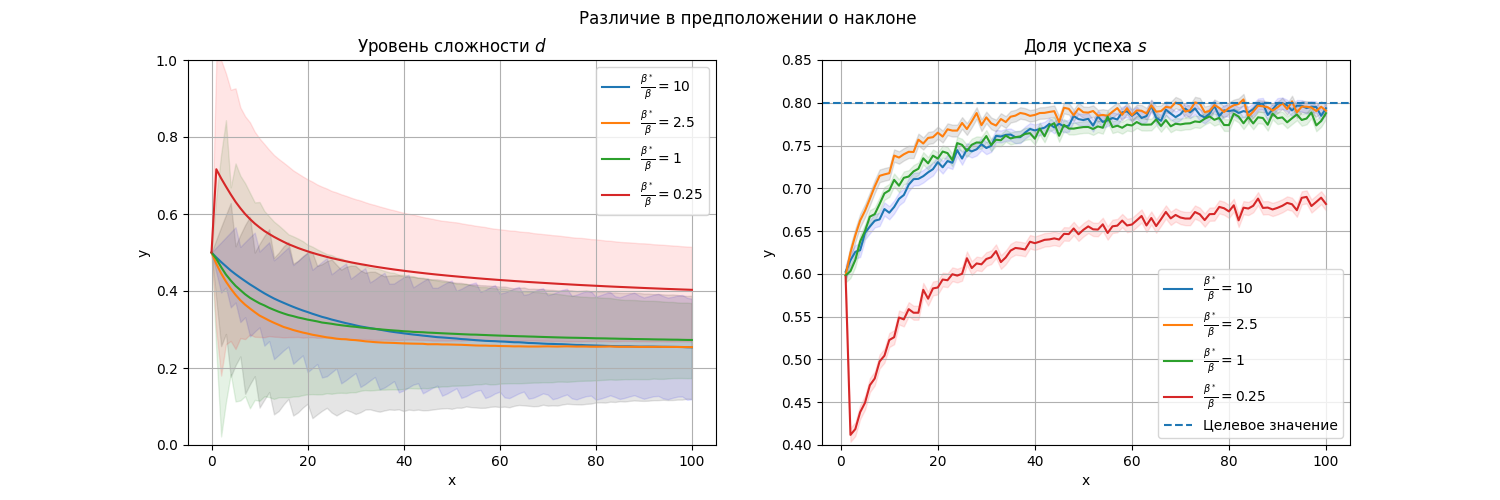
\includegraphics[width=0.9\textwidth]{assets/3/slop_affect.png}
    \caption{Значительные различия в предположениях о наклоне логистической регрессии приводят к снижению эффективности алгоритма}
    \label{exp3:lose_effictivness}
\end{figure}
\begin{table}
    \centering
    \begin{tabular}{ ||c | c|| }
        \hline 
        \text{Название алгоритма} &  \text{Число шагов}\\
        \hline 
        \text{Адаптированный алгоритм Р.-М.} $\frac{\beta^*}{\beta}=10$  & $400  \pm 20$ \\  
        \text{Адаптированный алгоритм Р.-М.} $\frac{\beta^*}{\beta}=2.5$ & \text{Не сошелся} \\
        \text{Адаптированный алгоритм Р.-М.} $\frac{\beta^*}{\beta}=1$ & $250 \pm 30$ \\
        \text{Адаптированный алгоритм Р.-М.} $\frac{\beta^*}{\beta}=0.25$ & $200 \pm 35 $   \\
        \hline
    \end{tabular}
    \caption{Сравнение числа шагов сходимости в постановке различающихся априорных представлений о наклоне кривой от действительного}
    \label{exp3:table}
\end{table}
\subsection{Модификация скользящим средним}
Численно исследуем применимость метода скользящего среднего к предложенному алгоритму и алгоритму с постоянным шагом. 
\begin{figure}[h]
    \centering
    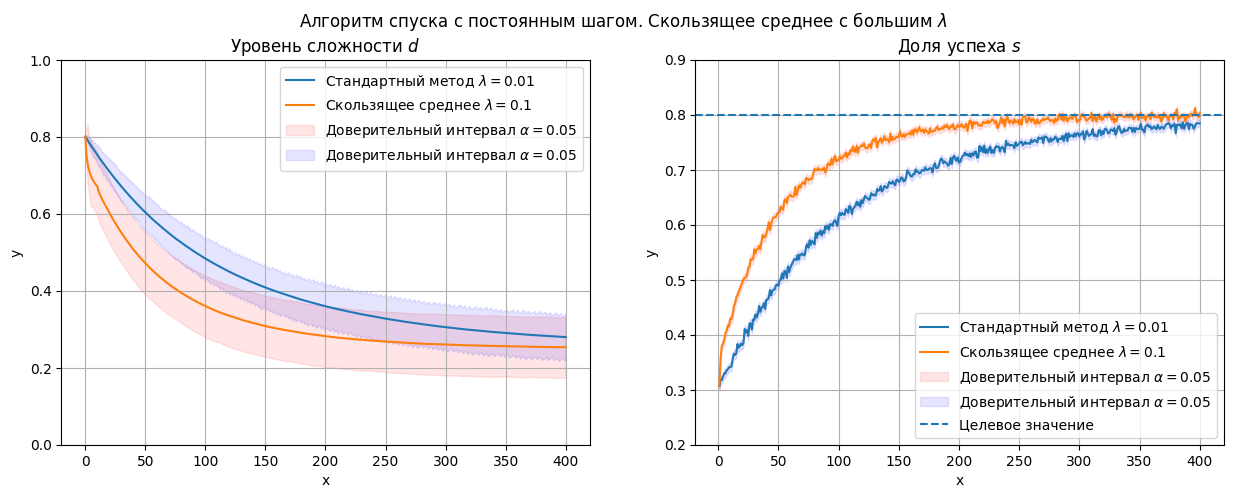
\includegraphics[width=0.9\textwidth]{assets/4/lambda_0.01_0.1.png}
    \caption{Метод скользящего среднего позволяет использовать больший параметр шага, не теряя устойчивость метода}
    \label{exp4:better_stability}
\end{figure}
\begin{figure}[h]
    \centering
    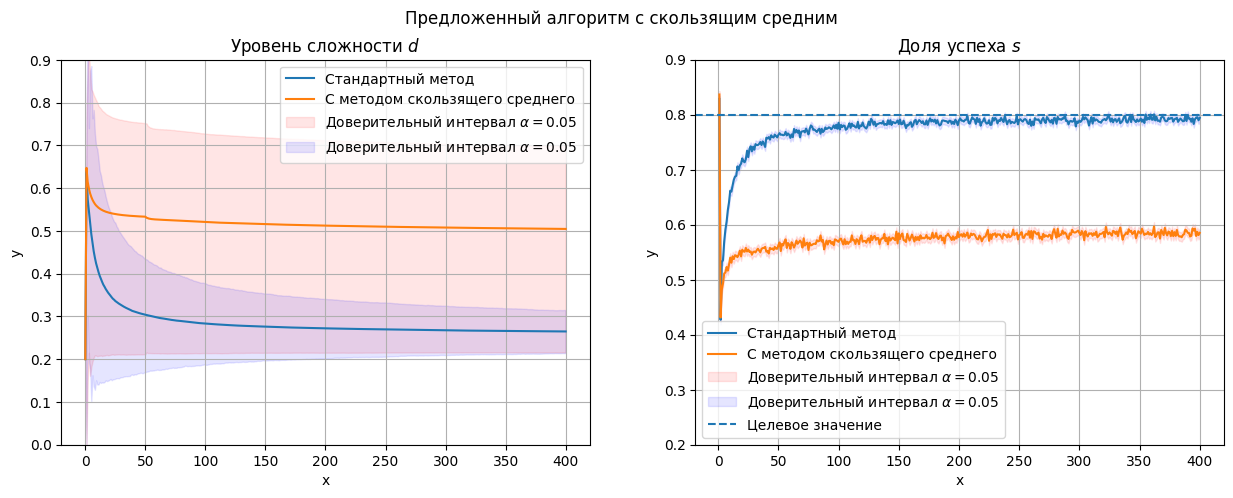
\includegraphics[width=0.9\textwidth]{assets/4/adaptive.png}
    \caption{Метод скользящего среднего не применим к предложенному алгоритму}
    \label{exp4:not_applied}
\end{figure}
\begin{table}
    \centering
    \begin{tabular}{ ||c | c|| }
        \hline
        \text{Название алгоритма} &  \text{Число шагов}\\
        \hline 
        \text{Алгоритм Р.-М. со скользящим средним $\lambda=0.01$} & \text{Не сошелся} \\
        \text{Алгоритм Р.-М. со скользящим средним $\lambda=0.1$} & $250\pm 40$  \\
        \text{Адаптированный алгоритм  Р.-М. со скользящим средним } & \text{Не сошелся}\\
        \hline 
    \end{tabular}
    \caption{Сравнение числа шагов с применением метода скользящего среднего}
    \label{exp4:table}
\end{table}

Расходимость предложенного метода связана с нарушениями условий \ref{polyak_assumptions}.

Таким образом, метод скользящего среднего \begin{enumerate}
    \item позволяет использовать больший шаг для обеспечения большей скорости сходимости
    \item не применим к предложенному алгоритму
\end{enumerate}

\section{Итоги}
Исследована постановка алгоритма Роббинса-Монро в условиях отклика, представленной случайной бернуллевской величины. 
Для случая ответа в виде логистической функции получен адаптивный численный алгоритм.К его ключевые преимуществам можно отнести:
\begin{itemize}
    \item оптимальную скорость сходимости при выполнение условий теоремы \ref{algo}
    \item стабильную дисперсию $s$ и $d$ на всех шагах оптимизации
    \item работу с естественными параметрами логистического распределения на всем интервале оптимизации. Это обстоятельство выгодно выделяет метод от классических методов, требующих подбора шага оптимизации.
\end{itemize}
Тем не менее алгоритм требует выбора априорных представлений о наклоне функции логистического распределения \ref{exp3:lose_effictivness}. Выполнить такой расчет можно на экспериментальных данных, использовав 
в качестве бинарного классификатора логистическую регрессию.

\subsection{Аппендикс}
\textit{Доказательство теоремы Роббинса-Монро} \label{monro}
Следуя доказательству \cite{blum1954approximation}, используем рекуррентную схема связи между ошибками на каждом шаге алгоритма $b_1,\dots,b_n$. 
В этом случае правило обновления Роббинса-Монро запишется как: 
\begin{equation}
    \mathrm{E_{x_t \sim p(x|s(d))}}(d_n+a_t(s^*-x_t) -d^*)^2.
\end{equation}
Раскрываем квадрат разности:
\begin{equation}
    (d_n - d^*)^2 + a_t^2 \mathrm{E_{x_t \sim p(x|s(d))}} (s^*-x_t)^2 - 2 a_t \mathrm{E_{x_t \sim p(x|s(d))}}\left[ (s^*-x_t)(d_n-d^*) \right].
\end{equation}
Используем несмещенность оценки $\mathrm{E}_{x \sim p(x|s)} x = s$:
\begin{equation}
    d_n =2 a_t (s^* -s(d))(d_n-d^*).
\end{equation}
Положительна, исходя из монотонности:
\begin{equation}
    \lim_{n \rightarrow \infty} b_n = b_1 + \sum_{j=1}^\infty a_n^2 c_n -2 \sum_1^{\infty} a_n d_n < \infty.
\end{equation}
Сходимость обоснуем через два последовательных шага: \begin{itemize}
    \item  $\sum_{j=1}^\infty a_n^2 c_n < \infty$ , поскольку при $\sum_{j=1} a_n^2 < \infty $ и $c_n$ -ограничены.
    \item $\sum_{j=1}^\infty a_n d_n < \sum_{j=1}^\infty a_n^2 c_n$,  т.к $b_n \ge 0$.
\end{itemize}
Покажем, что $\lim_{n \rightarrow \infty}{b_n}$  нулю следует из$\sum_{j=1}^\infty a_j  =\infty$ .
Действительно, зададим ряд $m_n = \frac{b_n}{d_n}$, т.к. он неотрицателен, то $\sum_{i=1}^{\infty} a_n k_n = \infty $. 
Тогда $\sum_{.i=1}^{\infty} a_n k_n b_N < \infty $. 
Из сходимости ряда из неотрицательных элементов следует, что $\lim_{n \rightarrow \infty}b_n =0$.
$\blacksquare$

\textit{Случай $b_n \ne s^*$} \label{ino}
Общая схема доказательства приведена в \cite{lai1979adaptive}.
$\blacksquare$

\printbibliography


\pagebreak

\subsection{Приложение}

\subsubsection{Эксперимент 1}
\begin{figure}[h!]
    \centering
    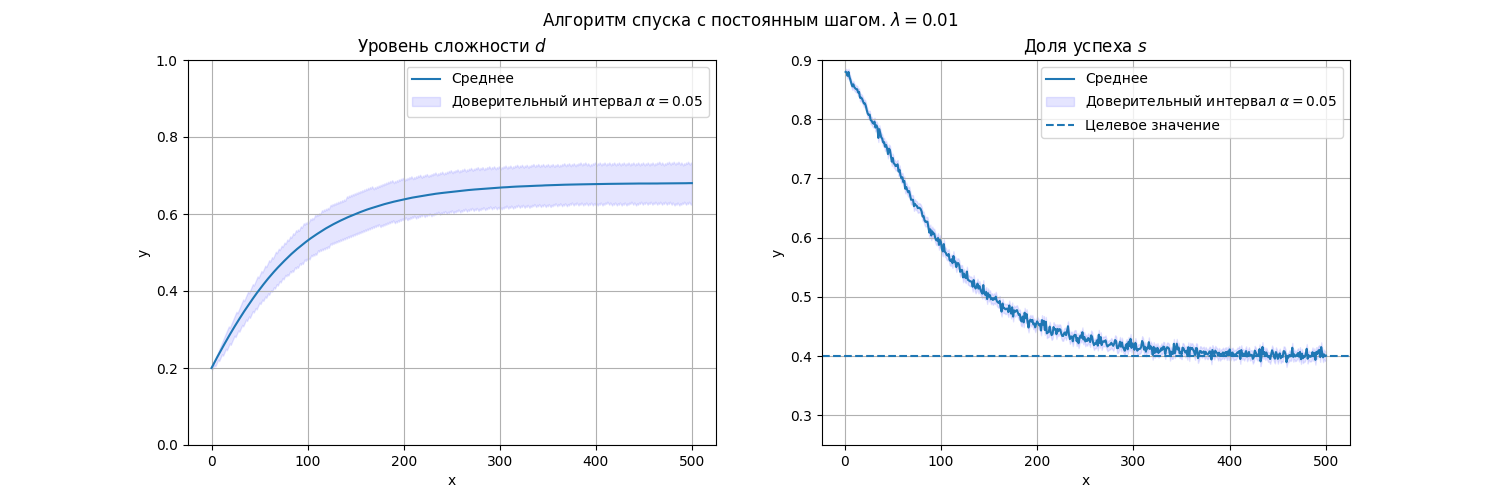
\includegraphics[width=0.8\textwidth]{assets/1/fixed.png}
    % \caption{Фиксированный $a_n$. $lambda =0.01$ }
    \label{exp1:fixed}
\end{figure}
\begin{figure}[h!]
    \centering
    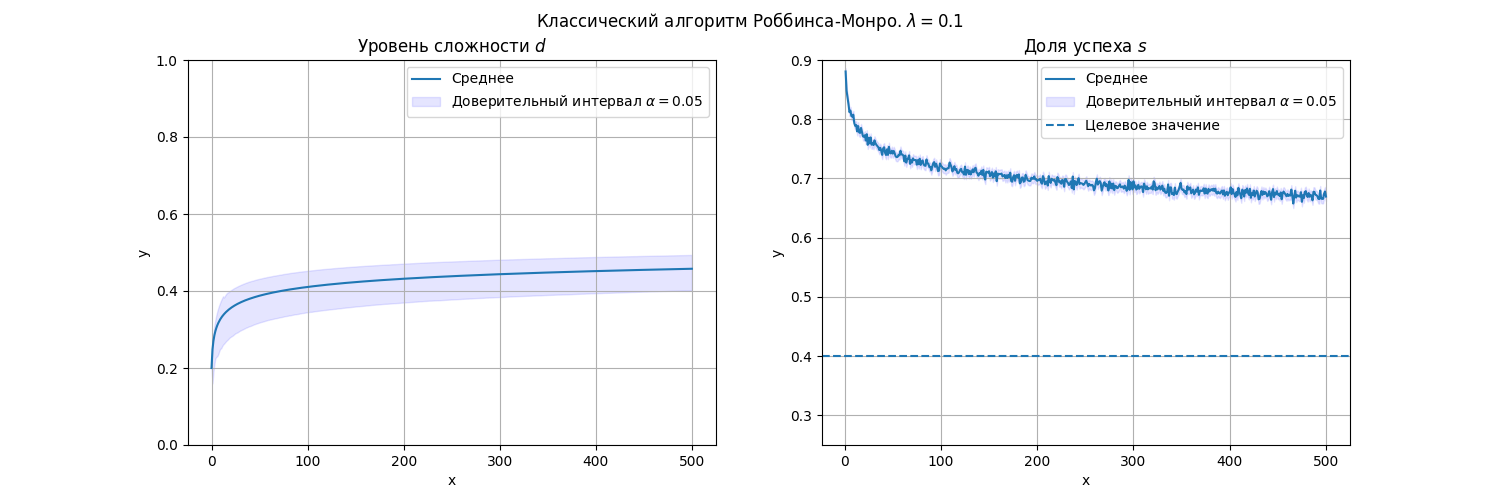
\includegraphics[width=0.8\textwidth]{assets/1/lambda_0.1.png}
    % \caption{Классический Роббинса-Монро.$lambda =0.1$ }
    \label{exp1:lambda_0.1}
\end{figure}
\begin{figure}[h!]
    \centering
    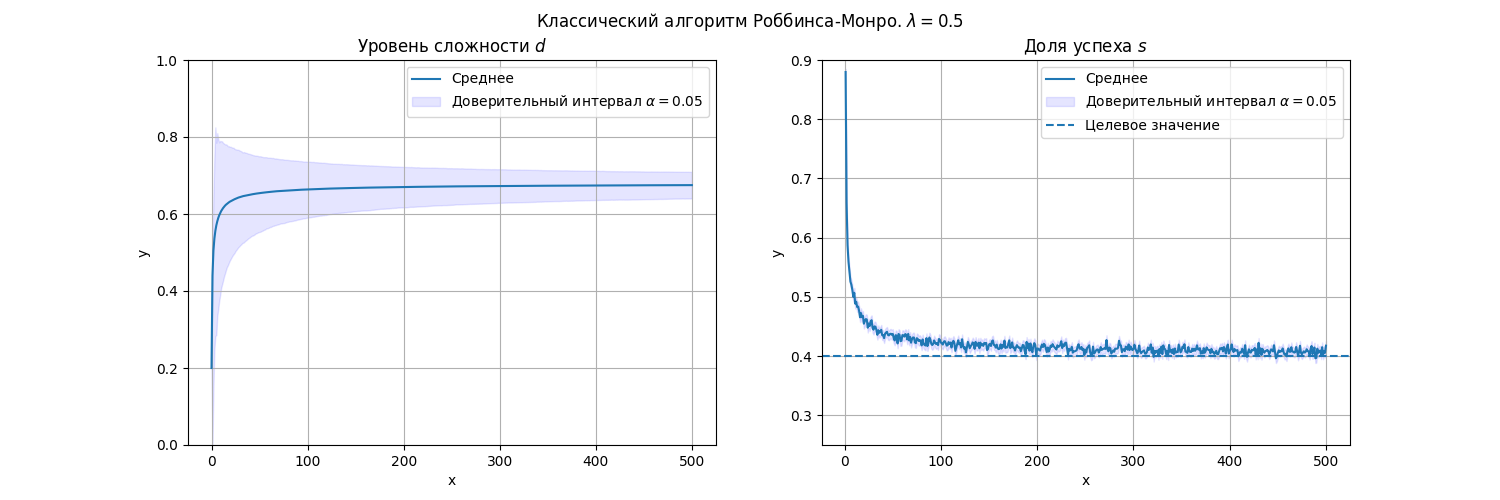
\includegraphics[width=0.8\textwidth]{assets/1/lambda_0.5.png}
    % \caption{Классический Роббинса-Монро.$lambda =0.5$ }
    \label{exp1:lambda_0.5}
\end{figure}
\begin{figure}[h!]
    \centering
    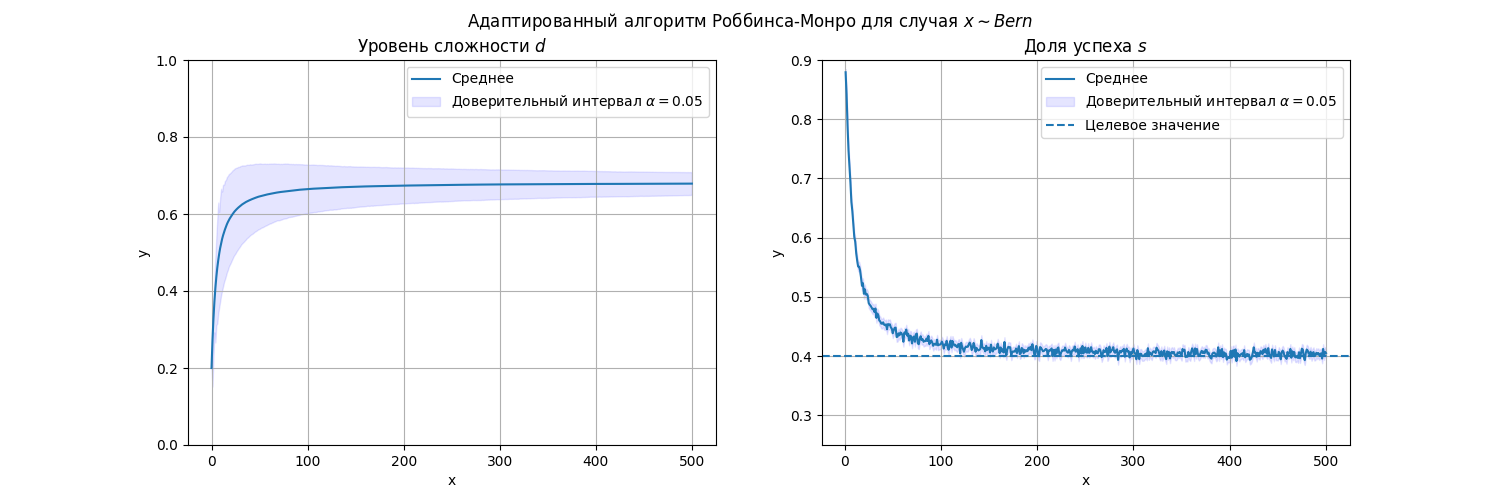
\includegraphics[width=0.8\textwidth]{assets/1/adaptive.png}
    % \caption{Предложенный алгоритм}
    \label{exp1:adaptive}
\end{figure}
\pagebreak
\subsubsection{Эксперимент 2}
\begin{figure}[h!]
    \centering
    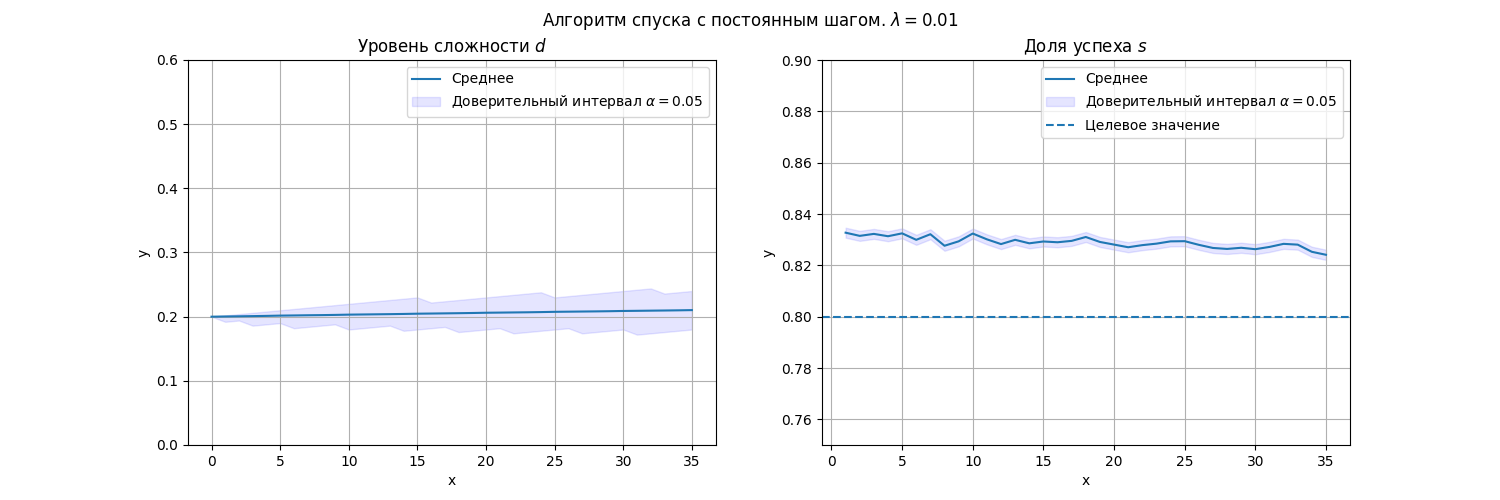
\includegraphics[width=0.8\textwidth]{assets/2/fixed.png}
    % \caption{Фиксированный $a_n$. $lambda =0.01$ }
    \label{exp2:fixed}
\end{figure}
\begin{figure}[h!]
    \centering
    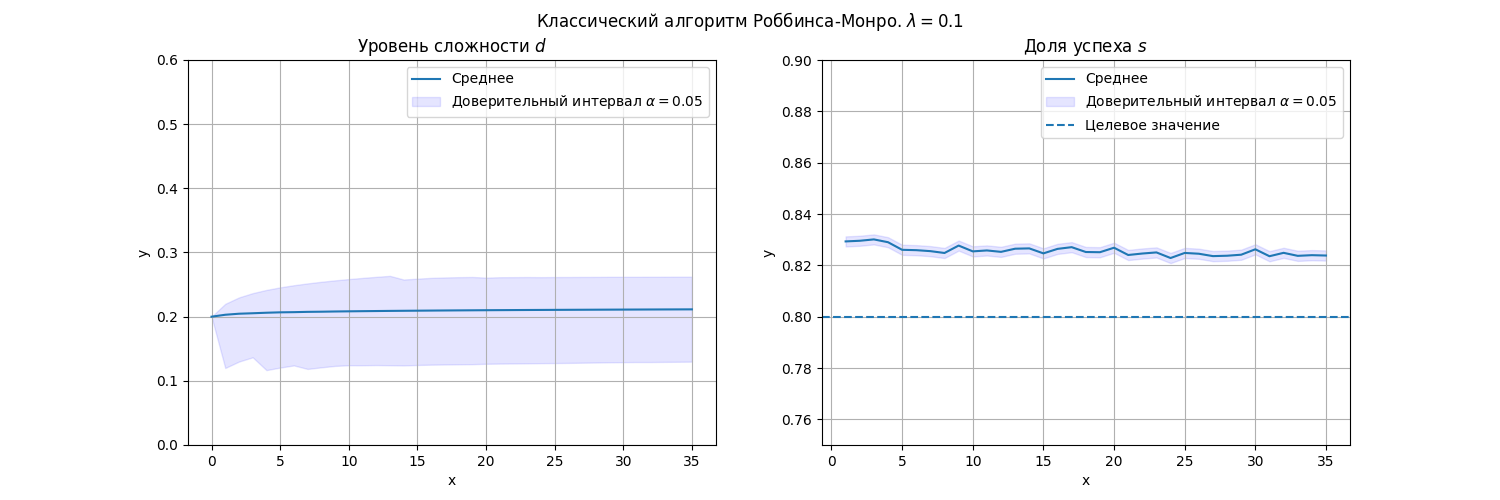
\includegraphics[width=0.8\textwidth]{assets/2/lambda_0.1.png}
    % \caption{Классический Роббинса-Монро.$lambda =0.1$ }
    \label{exp2:lambda_0.1}
\end{figure}
\begin{figure}[h!]
    \centering
    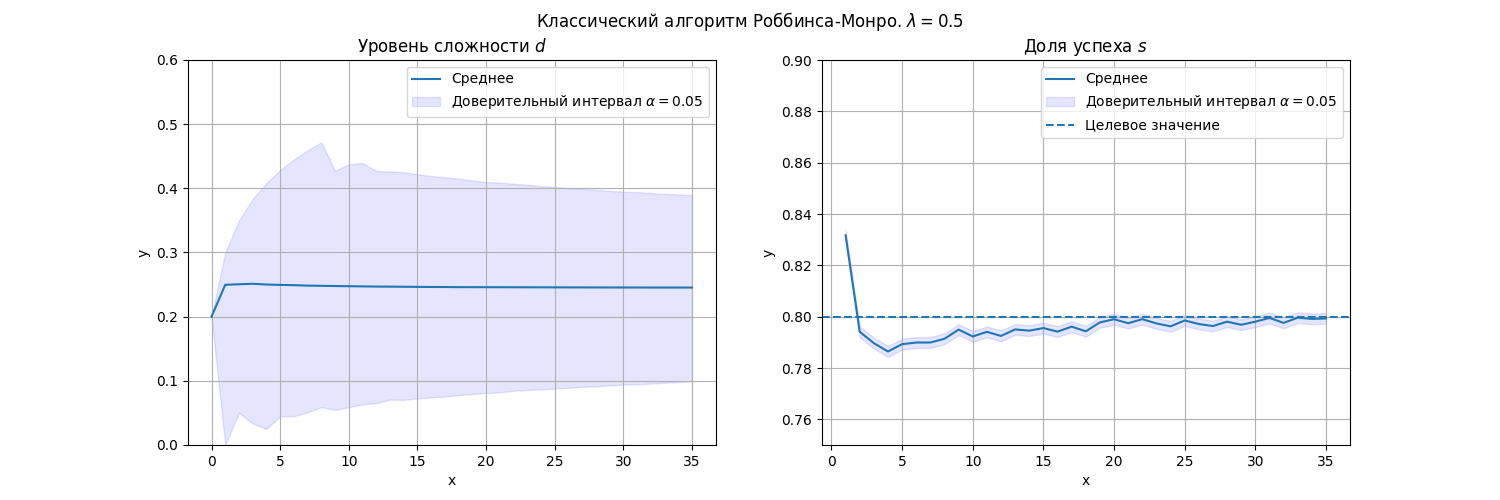
\includegraphics[width=0.8\textwidth]{assets/2/lambda_0.5.png}
    % \caption{Классический Роббинса-Монро.$lambda =0.5$ }
    \label{exp2:lambda_0.5}
\end{figure}
\begin{figure}[h!]
    \centering
    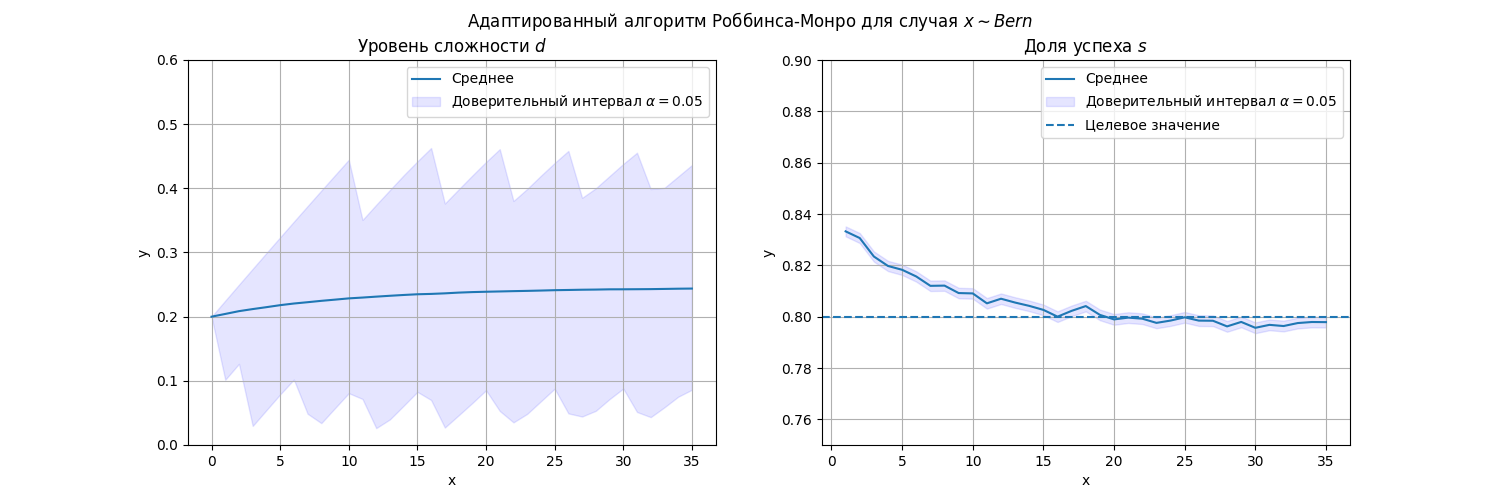
\includegraphics[width=0.8\textwidth]{assets/2/adaptive.png}
    % \caption{Предложенный алгоритм}
    \label{exp2:adaptive}
\end{figure}
\pagebreak
\subsubsection{Эксперимент 3}
\begin{figure}[h!]
    \centering
    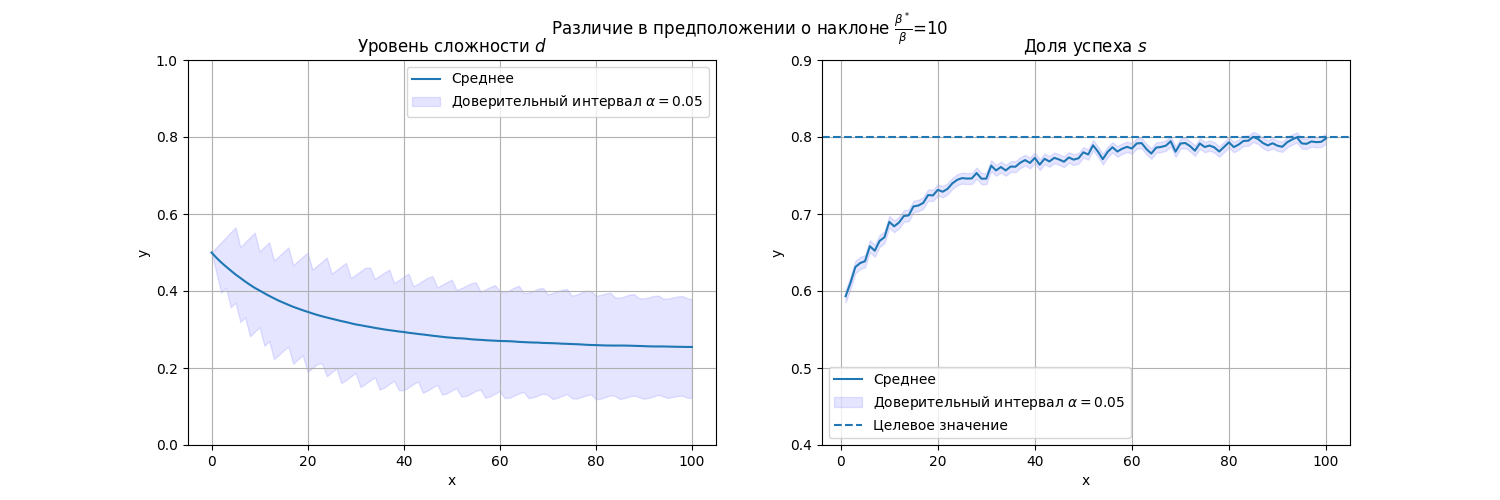
\includegraphics[width=0.8\textwidth]{assets/3/0.png}
     % \caption{Предложенный алгоритм}
    \label{exp3:10}
\end{figure}
\begin{figure}[h!]
    \centering
    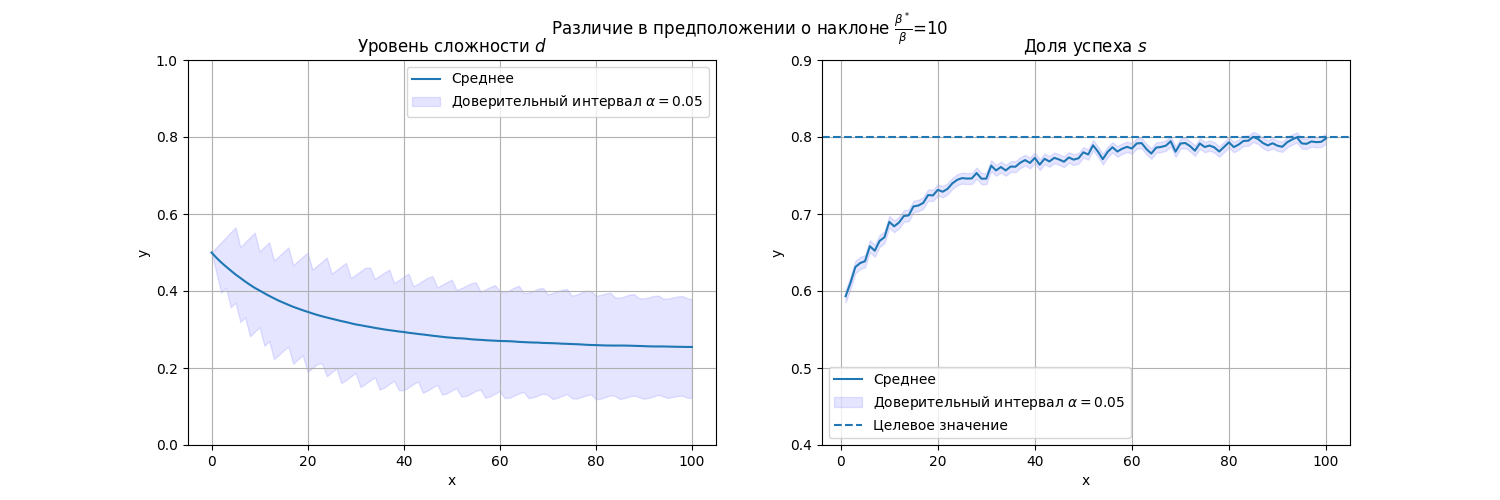
\includegraphics[width=0.8\textwidth]{assets/3/0.png}
    \label{exp3:2_5}
\end{figure}
\begin{figure}[h!]
    \centering
    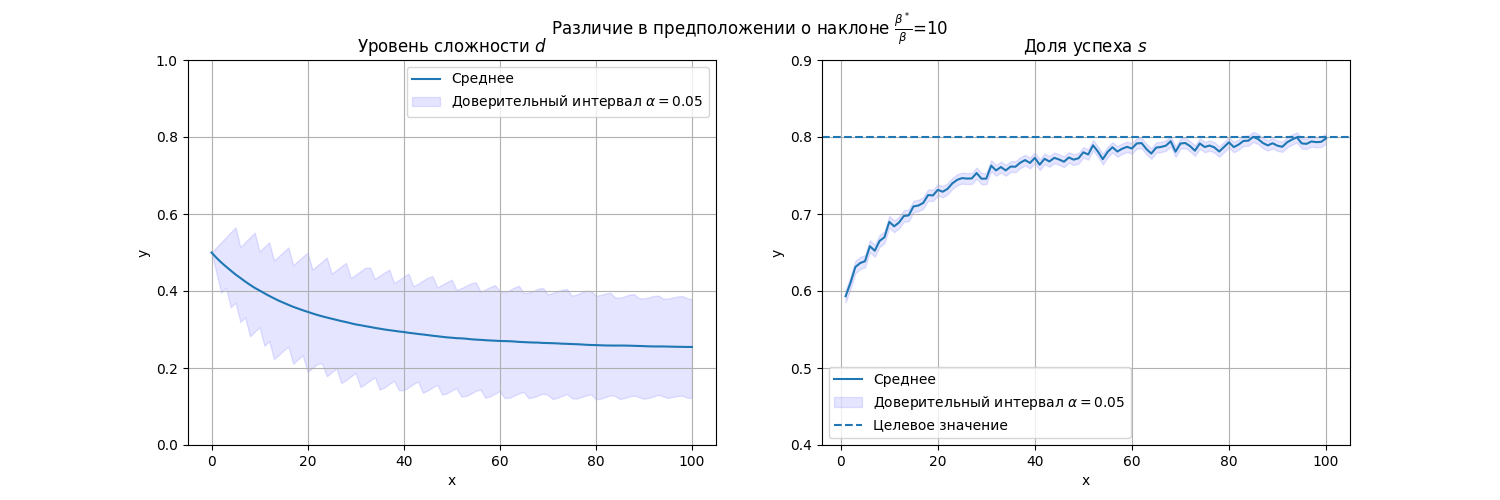
\includegraphics[width=0.8\textwidth]{assets/3/0.png}
    \label{exp3:1}
\end{figure}
\begin{figure}[h!]
    \centering
    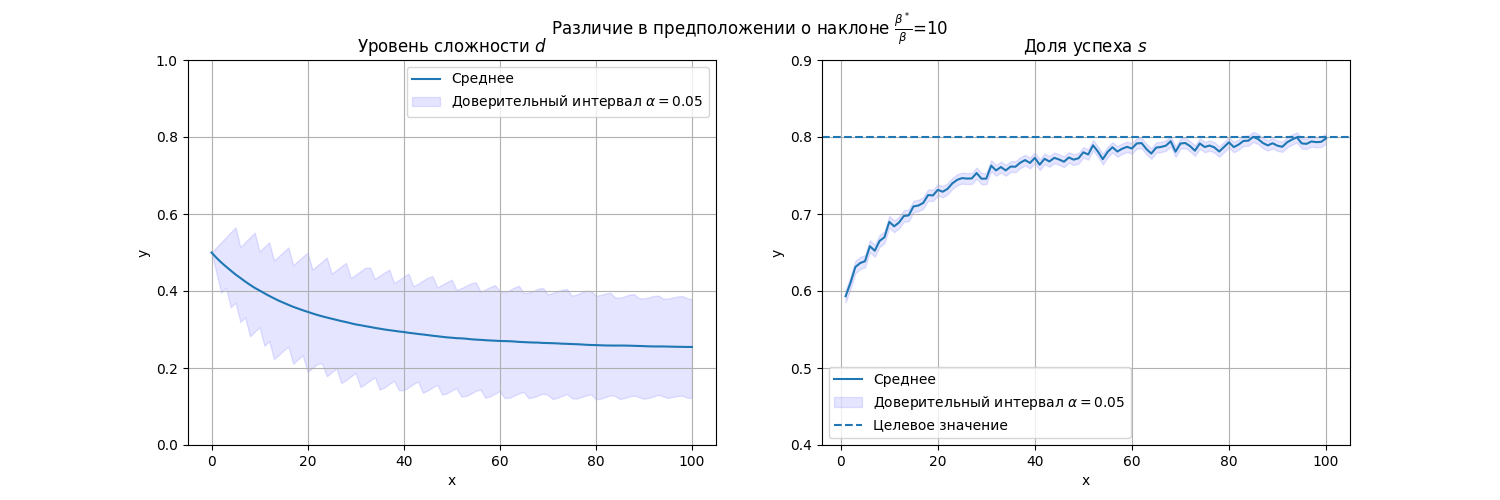
\includegraphics[width=0.8\textwidth]{assets/3/0.png}
    \label{exp3:_0.25}
\end{figure}
\pagebreak
\subsubsection{Эксперимент 4}
\begin{figure}[h!]
    \centering
    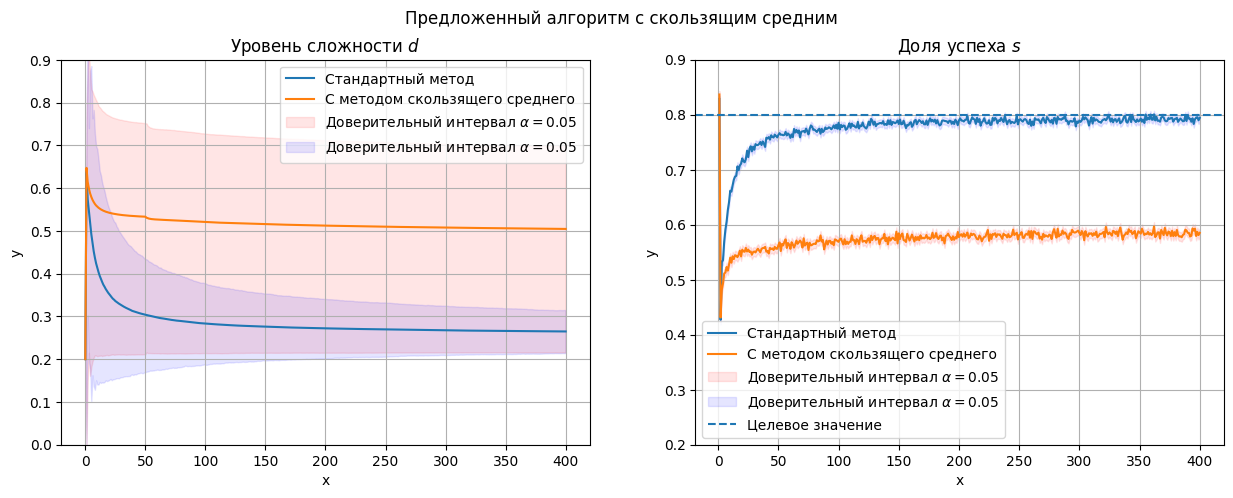
\includegraphics[width=0.8\textwidth]{assets/4/adaptive.png}
    % \caption{Предложенный алгоритм}
    \label{exp4:algo}
\end{figure}
\end{document}
